\cite{mvc-paper} apresenta uma proposta para lidar com conjuntos de dados grandes e complexos dentro de uma aplicação, enquanto permite que a interface de usuário seja atualizada conforme as alterações ocorrem.
São apresentados três componentes principais: \emph{Model} (modelo), \emph{View} (visualizador) e \emph{Controller} (controlador).

A \emph{Model} é representada como uma estrutura de dados unificada com os métodos necessários para manipulá-los.
Serviços externos, como APIs e bancos de dados podem ser consumidos por ela.
Dada uma \emph{Model} qualquer, há uma ou mais \emph{Views} associadas a ela, capazes de exibir alguma representação gráfica ou textual da \emph{Model} em questão.
A \emph{View} pode consultar a \emph{Model} para decidir sobre a exibição dos dados.
O \emph{Controller} é a ponte entre o usuário e uma ou mais \emph{Views}.
Ele é responsável por validar e adequar a entrada do usuário à \emph{Model}, e repassar o resultado do processamento para as \emph{Views} correspondentes.
A Figura~\ref{fig:mvc} apresenta um diagrama que ilustra o funcionamento do padrão MVC.

\begin{figure}[ht]
	\centering
	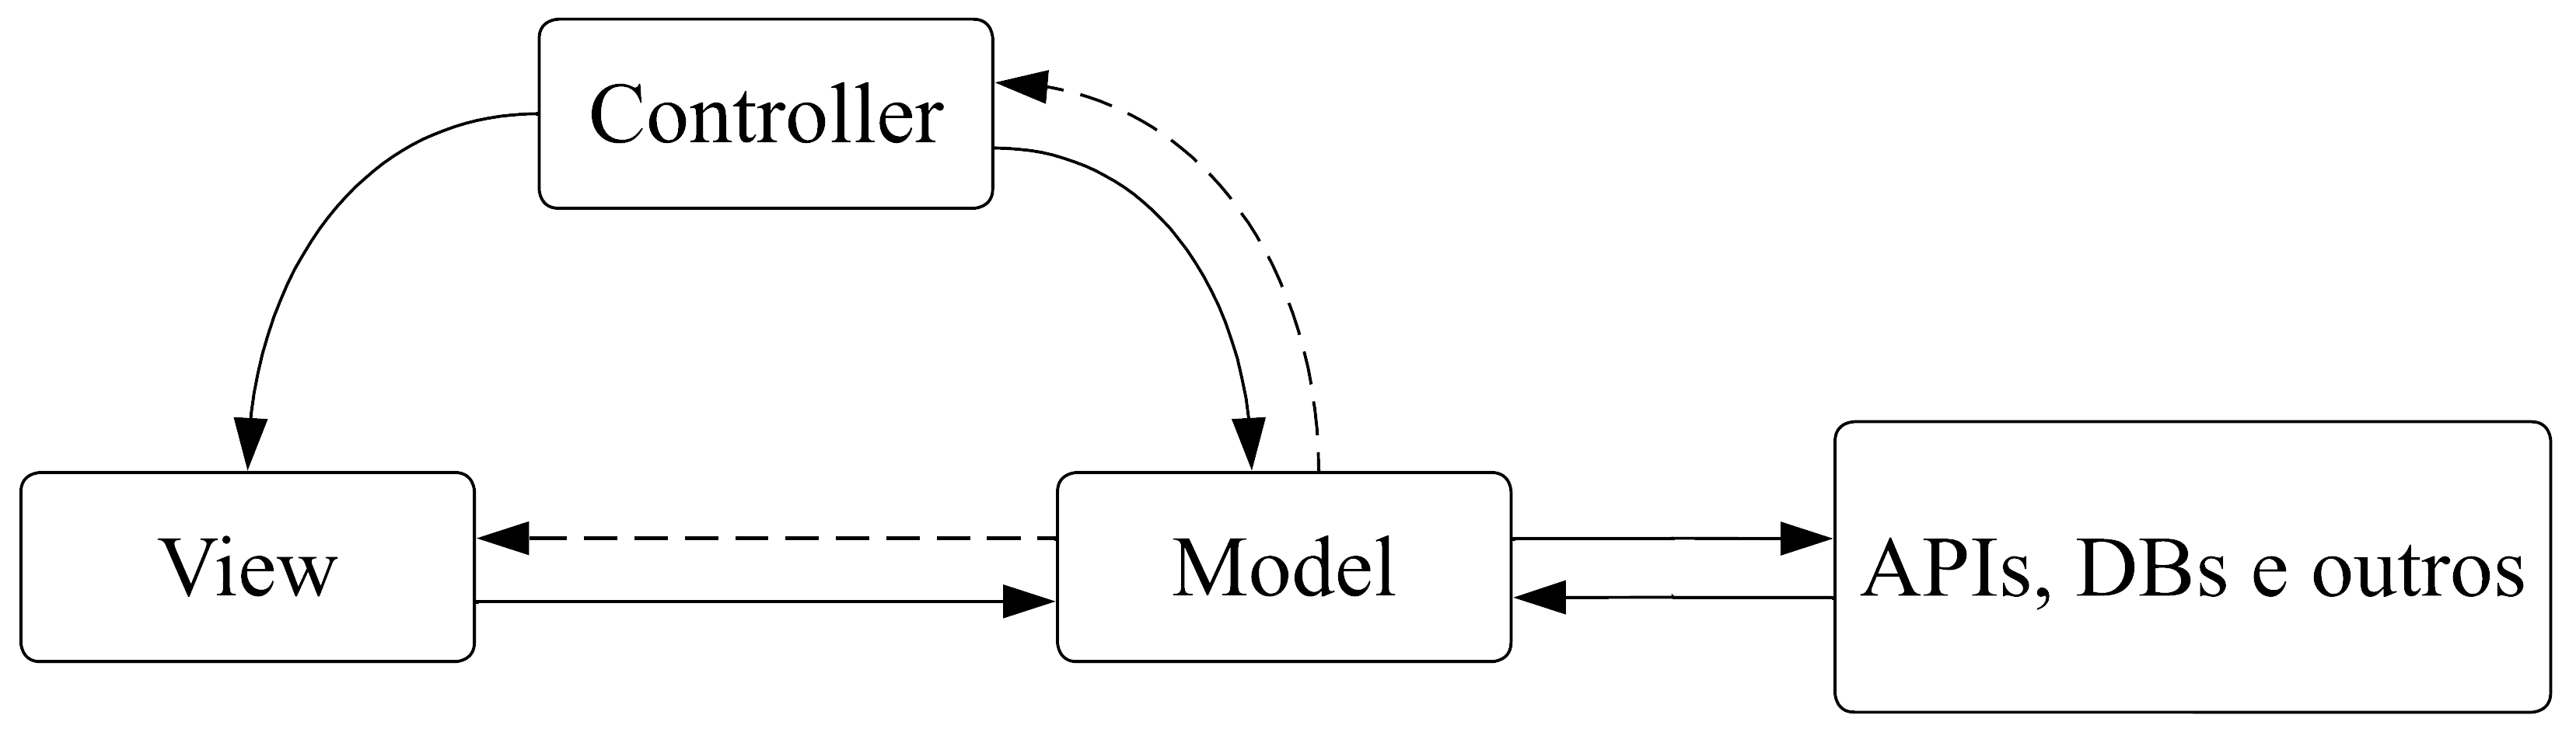
\includegraphics[width=0.52\textwidth]{images/mvc.png}
	\caption{Diagrama do padrão MVC}
	\label{fig:mvc}
\end{figure}